%-%-%-%-%-%-%-%-%-%-%-%-%-%-%-%-%-%-%-%-%-%-%-%-%-%-%-%-%-%-%-%-%-%-%-%-%-%-%
%%% MAIN DOCUMENT %%%

%-%-%-%-%-%-%-%-%-%-%-%-%-%-%-%-%-%-%-%-%-%-%-%-%-%-%-%-%-%-%-%-%-%-%-%-%-%-%

\documentclass[12pt, oneside]{book}
% \usepackage{C:/Users/paulb/VSTeX/local/draculatheme}
% \usepackage[T1]{fontenc}


%%% AESTHETICS %%%
%-%-%-%-%-%-%-%-%-%-%-%-%-%-%-%-%-%-%-%-%-%-%-%-%-%-%-%-%-%-%-%-%-%-%-%-%-%-%


%%% Dimensions and Spacing %%%
\usepackage[margin=1in]{geometry}
\usepackage{setspace}
\linespread{1}
\usepackage{listings}
\usepackage{pdflscape}
\usepackage{tikz}
\usetikzlibrary{shapes,backgrounds,calc,patterns,positioning,decorations.pathmorphing}
\usepgflibrary{shadings}
\usepackage[framemethod=tikz]{mdframed}
\usepackage{mathrsfs}
\usepackage{changepage}
\usepackage{multicol}
\usepackage{amsfonts}
\usepackage{amssymb}
\usepackage{multirow}
\usepackage{slashed}
\usepackage{enumerate}
\usepackage{booktabs}
\usepackage{tasks}
\usepackage{enumitem}
\usepackage{kantlipsum}  %This package lets us generate random text for example purposes.



%%% Define new colors %%%
\usepackage{xcolor}
\definecolor{orangehdx}{rgb}{0.96, 0.51, 0.16}
% \colorlet{firstlevel}{orangehdx}
% \colorlet{secondlevel}{orangehdx!80!black}
% \colorlet{thirdlevel}{orangehdx!60!black}
% \colorlet{fourthlevel}{orangehdx!40!black}
% \colorlet{fifthlevel}{orangehdx!20!black}
% \colorlet{sixthlevel}{orangehdx!10!black}



% Normal colors
\definecolor{xred}{HTML}{BD4242}
\definecolor{xblue}{HTML}{4268BD}
\definecolor{xgreen}{HTML}{52B256}
\definecolor{xpurple}{HTML}{7F52B2}
\definecolor{xorange}{HTML}{FD9337}
\definecolor{xdotted}{HTML}{999999}
\definecolor{xgray}{HTML}{777777}
\definecolor{xcyan}{HTML}{80F5DC}
\definecolor{xpink}{HTML}{F690EA}
\definecolor{xgrayblue}{HTML}{49B095}
\definecolor{xgraycyan}{HTML}{5AA1B9}

% Dark colors
\colorlet{xdarkred}{red!85!black}
\colorlet{xdarkblue}{xblue!85!black}
\colorlet{xdarkgreen}{xgreen!85!black}
\colorlet{xdarkpurple}{xpurple!85!black}
\colorlet{xdarkorange}{xorange!85!black}
\definecolor{xdarkcyan}{HTML}{008B8B}
\colorlet{xdarkgray}{xgray!85!black}

% Very dark colors
\colorlet{xverydarkblue}{xblue!50!black}

% Document-specific colors
\colorlet{normaltextcolor}{black}
\colorlet{figtextcolor}{xblue}

% Enumerated colors
\colorlet{xcol0}{black}
\colorlet{xcol1}{xred}
\colorlet{xcol2}{xblue}
\colorlet{xcol3}{xgreen}
\colorlet{xcol4}{xpurple}
\colorlet{xcol5}{xorange}
\colorlet{xcol6}{xcyan}
\colorlet{xcol7}{xpink!75!black}

% Blue-Purple (should just used colorbrewer...)
\definecolor{xrainbow0}{HTML}{e41a1c}
\definecolor{xrainbow1}{HTML}{a24057}
\definecolor{xrainbow2}{HTML}{606692}
\definecolor{xrainbow3}{HTML}{3a85a8}
\definecolor{xrainbow4}{HTML}{42977e}
\definecolor{xrainbow5}{HTML}{4aaa54}
\definecolor{xrainbow6}{HTML}{629363}
\definecolor{xrainbow7}{HTML}{7e6e85}
\definecolor{xrainbow8}{HTML}{9c509b}
\definecolor{xrainbow9}{HTML}{c4625d}
\definecolor{xrainbow10}{HTML}{eb751f}
\definecolor{xrainbow11}{HTML}{ff9709}

\definecolor{brainbackground}{HTML}{0d1f47}


\colorlet{firstlevel}{xrainbow1}
\colorlet{secondlevel}{xrainbow2}
\colorlet{thirdlevel}{xrainbow3}
\colorlet{fourthlevel}{xrainbow4}
\colorlet{fifthlevel}{xrainbow5}
\colorlet{sixthlevel}{xrainbow6}
\colorlet{seventhlevel}{xrainbow7}
\colorlet{eighthlevel}{xrainbow8}
\colorlet{ninthlevel}{xrainbow9}


\newcommand{\custombullet}[1]{%
    \tikz[baseline=-.75ex]{\node[circle, fill=#1, inner sep=1.5pt] {};}%
}

\setlistdepth{9}

% Create a custom list environment
\newlist{coloredlist}{itemize}{9}
\setlist[coloredlist,1]{label=\custombullet{firstlevel}}
\setlist[coloredlist,2]{label=\custombullet{secondlevel}}
\setlist[coloredlist,3]{label=\custombullet{thirdlevel}}
\setlist[coloredlist,4]{label=\custombullet{fourthlevel}}
\setlist[coloredlist,5]{label=\custombullet{fifthlevel}}
\setlist[coloredlist,6]{label=\custombullet{sixthlevel}}
\setlist[coloredlist,7]{label=\custombullet{seventhlevel}}
\setlist[coloredlist,8]{label=\custombullet{eighthlevel}}
\setlist[coloredlist,9]{label=\custombullet{ninthlevel}}


%------- %
% XHFILL %
%------- %



%%% Chapter Headings %%%

\newcommand{\gradientrule}{
    \begin{tikzpicture}
        \shade[left color=orangehdx, right color=black, middle color=gray] (0,0) rectangle (\linewidth,0.4pt);
    \end{tikzpicture}
}

\usepackage[Glenn]{fncychap}
% \ChTitleVar{\bfseries\scshape\color{draculafg}} % Needed for Dracula theme
% \ChNumVar{\large\selectfont\color{draculafg}} % Needed for Dracula theme
% \ChNameVar{\large\color{draculafg}} % Needed for Dracula theme
\ChTitleVar{\bfseries\scshape\color{black}}
\ChNumVar{\large\selectfont\color{black}}
\ChNameVar{\large\color{black}}
\usepackage{xpatch}

% \xpatchcmd{\DOCH}
%   {\mghrulefill}{\gradientrule\mghrulefill}
%   {}{\PatchFailed}
% \xpatchcmd{\DOTI}
%   {\mghrulefill}{\gradientrule\mghrulefill}
%   {}{\PatchFailed}
% \xpatchcmd{\DOTIS}
%   {\mghrulefill}{\gradientrule\mghrulefill}
%   {}{\PatchFailed}

\xpatchcmd\DOCH
{\mghrulefill}{\color{orangehdx}\mghrulefill}
{}{\PatchFailed}
\xpatchcmd\DOTI
{\mghrulefill}{\color{orangehdx}\mghrulefill}
{}{\PatchFailed}
\xpatchcmd\DOTIS
{\mghrulefill}{\color{orangehdx}\mghrulefill}
{}{\PatchFailed}


% \usepackage[Bjornstrup]{fncychap}

% \newcommand{\gradient}[1]{
% \begin{tikzpicture}
%     \node (rect) at (0,0) [fill=blue,,path fading=East,minimum width=\linewidth,minimum height=2.5cm] {};
%     \node(title)[above left = 10pt and 10pt of rect.south east, anchor=south east, font=\CTV] {\textcolor{horange}{#1}};
%     \ifnum \thechapter>0\node[left = 10pt of rect.north east,  anchor=center, font=\CNoV] {\textcolor{horange}{\thechapter}};\fi%
% \end{tikzpicture}%
% \vskip 40pt
% }


% \renewcommand{\DOCH}{}
% \renewcommand{\DOTI}[1]{\gradient{#1}}
% \renewcommand{\DOTIS}[1]{\gradient{#1}}

%% Change Chapter Heading Placement %%
\usepackage{etoolbox}
\makeatletter
\patchcmd{\@makechapterhead}{\vspace*{50\p@}}{\vspace*{-20\p@}}{}{}
\patchcmd{\@makeschapterhead}{\vspace*{50\p@}}{\vspace*{-20\p@}}{}{}
\patchcmd{\DOTI}{\vskip 80\p@}{\vskip 40\p@}{}{}
\patchcmd{\DOTIS}{\vskip 40\p@}{\vskip 0\p@}{}{}
\makeatother

% \usepackage[explicit]{titlesec}
% \newcommand*\chapterlabel{}\pmod
% \titleformat{\chapter}
%   {\gdef\chapterlabel{}
%    \normalfont\sffamily\Huge\bfseries\scshape}
%   {\gdef\chapterlabel{\thechapter\ }}{0pt}
%   {\begin{tikzpicture}[remember picture,overlay]
%     \node[yshift=-3cm] at (current page.north west)
%       {\begin{tikzpicture}[remember picture, overlay]
%         \draw[fill=LightSkyBlue] (0,0) rectangle
%           (\paperwidth,3cm);
%         \node[anchor=east,xshift=.9\paperwidth,rectangle,
%               sharp corners=downhill=20pt,inner sep=11pt,
%               fill=MidnightBlue]
%               {\color{white}\chapterlabel#1};
%        \end{tikzpicture}
%       };
%    \end{tikzpicture}
%   }
% \titlespacing*{\chapter}{0pt}{50pt}{-60pt}

% \usepackage[Conny]{fncychap}
% \usepackage[Rejne]{fncychap}
% \ChNameVar{\bfseries}  % Makes the chapter "Chapter #" bold
% \ChNumVar{\bfseries}   % Makes the chapter number bold
% \ChTitleVar{\bfseries} % Makes the chapter title bold
% % Define a custom color, for example:
% \definecolor{mycolor}{RGB}{0,128,255}

% % Redefine the chapter style in Rejne to change the line colors
% \makeatletter
% \ChRuleWidth{2pt}   % Change the thickness of the lines
% \renewcommand{\DOCH}{%
%   \vspace*{-50\p@}% Moves the chapter title up/down if needed
%   {\color{mycolor} \hrule \@chapapp{} \space \thechapter \hrule}% Customizes the chapter header with color
% }
% \renewcommand{\DOTI}[1]{%
%   \vskip 20\p@ % Adjusts the space above the title
%   \bfseries #1\par % Embolden the title
%   \vskip 20\p@ % Adjusts the space below the title
% }
% \makeatother

% %% Change Chapter Heading Placement %%
% \usepackage{etoolbox}
% \makeatletter
% \patchcmd{\@makechapterhead}{\vspace*{50\p@}}{\vspace*{-20\p@}}{}{}
% \patchcmd{\@makeschapterhead}{\vspace*{50\p@}}{\vspace*{-20\p@}}{}{}
% \patchcmd{\DOTI}{\vskip 80\p@}{\vskip 40\p@}{}{}
% \patchcmd{\DOTIS}{\vskip 40\p@}{\vskip 0\p@}{}{}
% \makeatother

\renewcommand{\thesection}{\thechapter.\arabic{section}} %% Chapter.Section Numbering


%%% FIGURES %%%
\usepackage{graphicx}  
\graphicspath{ {images/} }  
% \numberwithin{figure}{section}
\usepackage{float}
\usepackage{caption}

%%% Hyperlinks %%%
\usepackage{hyperref}
\definecolor{horange}{HTML}{f58026}
\hypersetup{
	colorlinks=true,
	linkcolor=horange,
	filecolor=horange,      
	urlcolor=horange,
}

\newcommand{\squigglyline}{%
  \noindent
  \tikz[baseline=-0.5ex]{
    \draw[decorate, decoration={snake, amplitude=0.5mm, segment length=3mm}] 
      (0,0) -- (\dimexpr\linewidth-.46in\relax,0);
  }%
}


%% Headers and Footers %%
\usepackage{fancyhdr} % This should be set AFTER setting up the page geometry
\pagestyle{fancy} % options: empty , plain , fancy
\renewcommand{\chaptermark}[1]{\markboth{\thechapter.\ #1}{}}
\fancyhead[R]{\leftmark}
\fancyhead[L]{Hendrix College}
\fancyhead[C]{
\includegraphics[height=.50cm]{images/small logo.png}}
% \fancyhead[C]{
\includegraphics[height=.50cm]{images/small logo_white.png}} % Use for Dracula
\usepackage{xpatch}
\xpretocmd\headrule{\color{orangehdx}}{}{\PatchFailed}
\setlength{\footskip}{0.5in}
\setlength{\headheight}{18.5764pt}


%%%%% Colored Boxes %%%%%
\usepackage{tcolorbox}
\tcbuselibrary{skins}
\tcbuselibrary{theorems}
\tcbuselibrary{minted}
\newcounter{BoxCounter}


\newtcolorbox{note}{colback=black!15!white, colframe=black, boxrule=0.5mm, arc=4mm, left=4mm, right=4mm, top=2mm, bottom=2mm}

\newcommand{\cyanit}[1]{\textit{\textcolor{cyan}{#1}}}

%% Definitions %%
\newtcolorbox{wordbox}[1][]{%
enhanced,
sharp corners=downhill,
    colframe=black,
    colback=gray!15,
    coltitle=black,
    title={\large \textbf{Choices}},
    attach boxed title to top left={xshift=0.5cm},
    boxed title style={colback=white},
    #1
}

\let\cleardoublepage\clearpage


%-%-%-%-%-%-%-%-%-%-%-%-%-%-%-%-%-%-%-%-%-%-%-%-%-%-%-%-%-%-%-%-%-%-%-%-%-%-%

%% MATH PACKAGES, ENVIRONMENTS, COMMANDS %%
%-%-%-%-%-%-%-%-%-%-%-%-%-%-%-%-%-%-%-%-%-%-%-%-%-%-%-%-%-%-%-%-%-%-%-%-%-%-%
%You'll need your own packages, theorem types, and commands.




\newcommand{\pfs}{\noindent\makebox[\linewidth]{\rule{\textwidth}{0.4pt}}\vspace{0.5cm}}

% \newcommand{}{\marginnote{
\includegraphics[width=2em]{caution.png}}}


% end of preamble
%-%-%-%-%-%-%-%-%-%-%-%-%-%-%-%-%-%-%-%-%-%-%-%-%-%-%-%-%-%-%-%-%-%-%-%-%-%-%

\begin{document}

\numberwithin{BoxCounter}{section}


%-%-%-%-%-%-%-%-%-%-%-%-%-%-%-%-%-%-%-%-%-%-%-%-%-%-%-%-%-%-%-%-%-%-%-%-%-%-%
%%% COVER PAGE %%%
%-%-%-%-%-%-%-%-%-%-%-%-%-%-%-%-%-%-%-%-%-%-%-%-%-%-%-%-%-%-%-%-%-%-%-%-%-%-%

% Do not use all caps.
\newcommand{\titlestandin}[0]{Behavioral Neuroscience Notes}
\newcommand{\cussubtitle}[0]{PSYC 360}
% Date format should be like: "January 1, 2001"
\newcommand{\startdate}[0]{January 21, 2025}
\newcommand{\customenddate}[0]{May 14, 2025}
% Be sure to include degree recognition (e.g., B.S., M.S., Ph.D)
\newcommand{\professor}[0]{Prof. Jennifer Peszka, Ph.D.}

%-%-%-%-%-%-%-%-%-%-%-%-%-%-%-%-%-%-%-%-%-%-%-%-%-%-%-%-%



% \begin{titlepage}
%     \begin{center}

%         \vspace*{-2cm}
%         
\includegraphics[width=0.8\textwidth]{images/Hendrix Logo.png}\\
%         % 
\includegraphics[width=0.8\textwidth]{images/logo_white_text.png}\\ % Use for Dracula. Its the all white version of the logo.
%         \vfill

%         % Horizontal line above the title in 'horange' color
%         \textcolor{horange}{\rule{\textwidth}{1.0pt}}

%         \vspace{2em}

%         {\huge \textbf{\titlestandin}}

%         \vspace{1em} % Space between the title and the bottom line

%         \textcolor{horange}{\rule{\textwidth}{1.0pt}}

%         \vspace*{1\baselineskip}

%         {\LARGE \textbf{\cussubtitle}}

%         \begin{large}
%             \vspace*{2\baselineskip}

%             \textit{Start}  \\[1ex]
%             {\scshape \startdate} \\[0.3\baselineskip] % Year published

%             \vspace*{1\baselineskip}

%             \emph{Author} \\[1ex]
%             %Submitted by \\[\baselineskip]
%             {\Large Paul Beggs \\ \par} % Editor list
%             {\href{mailto:BeggsPA@Hendrix.edu}{{BeggsPA@Hendrix.edu}}}\\ % Editor affiliation

%             \vspace*{1\baselineskip}

%             \textit{Instructor} \\[1ex] % Tagline(s) or further description
%             \professor

%             \vspace*{1\baselineskip}

%             \textit{End}\\[1ex]
%             {\scshape  \customenddate} \\[0.3\baselineskip] % Year published

%             \thispagestyle{empty}

%         \end{large}
%     \end{center}
% \end{titlepage}
% \pagebreak


%-%-%-%-%-%-%-%-%-%-%-%-%-%-%-%-%-%-%-%-%-%-%-%-%-%-%-%-%-%-%-%-%-%-%-%-%-%-%

%%% Table of Contents %%%


% -%-%-%-%-%-%-%-%-%-%-%-%-%-%-%-%-%-%-%-%-%-%-%-%-%-%-%-%-%-%-%-%-%-%-%-%-%-%

% % Helper command to fix header for double paged ToC.
% % Temporarily adjust section marks for Table of Contents
% \begin{spacing}{1} % Can change spacing between entries in TOC
%     \renewcommand{\contentsname}{\Large\textbf{Table of Contents}} % Can rename here
%     \markboth{}{} % Clear the header marks for TOC
%     \pagestyle{fancy} % Ensure fancy style is active
%     \fancyhead[R]{Table of Contents} % Set TOC-specific header manually
%     \tableofcontents
%     \addtocontents{toc}{\protect\enlargethispage{\baselineskip}}
% \end{spacing}

% % Reset the headers to default for the rest of the document
% \fancyhead[R]{\leftmark}




% -%-%-%-%-%-%-%-%-%-%-%-%-%-%-%-%-%-%-%-%-%-%-%-%-%-%-%-%-%-%-%-%-%-%-%-%-%-%

\setcounter{chapter}{0}
\chapter{Origins of Behavioral Neuroscience}
\vspace*{-0.25in}
\section{Prehistoric}

\begin{coloredlist}
    \item A million years or more, people have been interested in the brain. Archaeological evidence shows that skulls are bashed in (jagged, not precise). As a result, the person dies, and therefore the brain is vital to life.
\end{coloredlist}

\section{7000 Years Ago}

\begin{coloredlist}
    \item New holes in the brain, but these holes show signs of healing. Therefore, these new holes are intended to help the person who is suffering.
    The fancy name is trephination.
    \item The theory for these holes is that they were drilled to cure the person. In other words, to relieve a person of a wicked spirit.
\end{coloredlist}

\section{5000 Years Ago}

\begin{coloredlist}
    \item \cyanit{Egyptian} physicians show that they were aware of brain damage through their writings.
    \item Complications arise because they thought the heart contained the soul--you need it to live and emotions effect it.
\end{coloredlist}

\section{Ancient Greece--4th Century, BC}

\label{person:hippocrates}%
\subsection{\cyanit{Hippocrates}}

\begin{coloredlist}
    \item Ponder the correlation between structure and function. Now, extend this thought to the brain/head.
    \item The brain is the place where sensation and intelligence reside. Not the heart.
\end{coloredlist}

\label{person:aristotle}%
\subsection{\cyanit{Aristotle}}

\begin{coloredlist}
    \item Clung to the idea of the heart being the one in charge.
    \item Figured the brain was a radiator. That is, we would send heated blood to the brain for it to be cooled off. This ``heated blood'' arose from our emotions. Thus, humans are more rational because we have a lot of cooling when compared to other animals.
\end{coloredlist}
\label{person:galen}%
\section{Roman Empire--\cyanit{Galen} 2nd Century, AD}

\begin{coloredlist}
    \item Galen is a physician to gladiators.
    \item Thought the cerebellum was for motor control (because the cerebellum is hard, like muscles) and the cerebrum is for memory because it is soft, and you can ``write on it.''
    \item Noticed there were large spaces (called ``ventricles,'' or ``spaces'') that were filled with fluid.
    \item From here, we get the four humors (fluids).
    \item Galen thought that these fluids are what control the brain, NOT the brain structure itself. Think of the purpose of canned vegetables. The tin container does not actively contribute to the liquid / vegetables; rather, it is disposable.
    \item These ideas were jumpstarted by the invention of aqueducts. The movement of water was so important from aqueducts, so the idea this idea was extended to the brain.
\end{coloredlist}

\section{Analysis by Analogy--17th Century}

\begin{coloredlist}
    \item \cyanit{French} developed hydraulically controlled machines.
    \item Again, this is adding to the idea that liquids (which can flow through things and cause movements) are responsible for the brain's functionality.
\end{coloredlist}
\label{person:descartes}%
\section{\cyanit{René Descartes}--1596-1650}

\begin{coloredlist}
    \item Believed that non-humans--what he called animals--are controlled by fluid.
    \item From this, he posited that the human body is a material entity functioning as a machine (like animals)--these are known as reflexes.
    \item But, the mind is nonmaterial and free from the laws of the universe and was uniquely human.
    \item Question: How does the nonmaterial part of the body (the mind) communicate with the material part of the body? Through the pineal gland! This gland would move around like a joystick and would manipulate the fluid that came from the third ventricle.
\end{coloredlist}

\section{The Mind/Body Problem}

\begin{coloredlist}
    \item What is the basic relationship between mental events and physical events?
    \item \cyanit{Dualism}--The mind exists independently of the brain and exerts some control over it.
    \item Strengths: Commonsense view.
    \item Weaknesses: The universe is composed of matter or energy.
    \item Modern neuroscientific explanation: Everything the body does rests on the events taking place in specific, definable parts of the nervous system--the ``mind'' is the product of the nervous system activity.
\end{coloredlist}

\section{The Scientific Method--17th and 18th Century}

\begin{coloredlist}
    \item A new world view at the end of the Renaissance.
    \begin{coloredlist}
        \item Replace \cyanit{Rationalism} with \cyanit{Scientific Method}.
    \end{coloredlist}
    \item Closer look at the substance of the brain:
    \begin{coloredlist}
        \item Gray and white matter change the way we look at the brain. That is, why would these parts of the brain that are clearly different, be different if the brain is used just to move fluids around.
        \item Also, everyone has the same brain structure, so these bumps and groves must mean something.
    \end{coloredlist}
\end{coloredlist}

\section{Electricity}

\begin{coloredlist}
    \item \label{person:newton}\cyanit{Isaac Newton} showed it is possible to electrically stimulate nerves.
    \item Then, \label{{person:galvani}} \cyanit{Luigi Galvani} and \label{person:bois-reymond}\cyanit{Emil du Bois-Reymond} showed that electricity can make muscles contract.
    \item Later on, \cyanit{Hermann von Helmholtz} showed that the speed of nerve conduction is not instantaneous.
    \item This important distinction shows that these nerves are not like wires--such as \cyanit{Luigi Galvani} and \cyanit{Emil du Bois-Reymond} thought.
    \item \cyanit{Bell} and \cyanit{Magendie} showed that the dorsal nerve root and the ventral nerve root are different.
    \item The dorsal nerve root is for sensory information, and the ventral nerve root is for motor information.
    \item \cyanit{Dorsal} = \cyanit{Sensory}: Think of the dorsal fin of a shark sensing vibrations in the water.
    \item \cyanit{Ventral} = \cyanit{Motor}: Think of a vent (like a car exhaust) pushing out movement.
    \item \cyanit{Johannes M\"uller} came up with the doctrine of \cyanit{Specific Nerve Energies}.
    \begin{coloredlist}
        \item This doctrine states that the nature of a sensation depends on which nerve is stimulated, not on how the nerve is stimulated.
        \item For example, if you stimulate the optic nerve, you will see something. If you stimulate the auditory nerve, you will hear something.
    \end{coloredlist}
    \item Spawned the \cyanit{Great Debate}: Is the brain a homogenous mass or is it made up of different parts?
\end{coloredlist}

\section{The Great Debate}

\begin{coloredlist}
    \item \cyanit{Franz Joseph Gall} and \cyanit{Johann Spurzheim} thought the bumps and groves on the head were due to the size of the brain parts.
    \item They concluded that the size of the brain parts was correlated to the use of that part.
    \item This is known as \cyanit{phrenology}.
    \item \cyanit{Localization of Functions}--brain function can be localized to regions, pathways, or neurons.
    \begin{coloredlist}
        \item Basically, if you cut out a piece of brain, and the animal (a pigeon) is no longer able to do a specific task, then that part of the brain is responsible for that task.
        \item However, it turns out that these pigeons were able to relearn the task, so the brain is not as localized as we thought (this research is from Flourens).
    \end{coloredlist}
    \item \cyanit{Aggregate Field Theory}--the brain is a homogenous mass.
    \begin{coloredlist}
        \item Complex brain functions emerge from the collective interactions of numerous simple neuronal activities.
        \item Unlike localizationist models, this theory emphasizes the distributed nature of cognitive processes across neural networks.
    \end{coloredlist}
    \item \cyanit{Pierre Flourens} (1794--1867)
    \begin{coloredlist}
        \item Studied the effect of brain damage with pigeons and supported the Aggregate Field Theory.
    \end{coloredlist}
    \item \cyanit{Paul Broca} (1824--1880)
    \begin{coloredlist}
        \item Found a patient who could understand language but could \cyanit{not speak}.
        \item After the patient died, Broca found a lesion in the \cyanit{left frontal lobe}.
        \item This area is now known as \cyanit{Broca's area}.
        \item This area is responsible for \cyanit{speech production}.
        \item These results put us back into the realm of Localization of Function.
    \end{coloredlist}
    \item In comes \cyanit{Carl Wernicke} (1874)
    \begin{coloredlist}
        \item Found a patient who could speak but could \cyanit{not understand} language.
        \item After the patient died, Wernicke found a lesion in the \cyanit{left temporal lobe}.
        \item This area is now known as \cyanit{Wernicke's area}.
        \item This area is responsible for \cyanit{language comprehension}.
    \end{coloredlist}
    \item Then, we have \cyanit{Gustav Fritsch} and \cyanit{Eduard Hitzig} (1870)
    \begin{coloredlist}
        \item Similarly to \cyanit{Luigi Galvani} and \cyanit{Emil du Bois-Reymond}, they electrically stimulated the brain.
        \item They found that the \cyanit{motor cortex} is responsible for \cyanit{movement}.
    \end{coloredlist}
    \item \cyanit{Shepherd Ivory Franz} (in D.C. from 1907--1924)
    \begin{coloredlist}
        \item Found that people are able to relearn tasks after brain damage.
    \end{coloredlist}
\end{coloredlist}

\section{Same Resolution?}

\begin{coloredlist}
    \item \cyanit{Modified Aggregate Field Theory}
    \begin{coloredlist}
        \item \cyanit{Karl S. Lashley} (1890-1958)
        \begin{coloredlist}
            \item \cyanit{The Principles of Mass Action}
            \begin{coloredlist}
                \item Complex behavior--such as learning--is dependent on the total mass of the brain.
            \end{coloredlist}
            \item \cyanit{Equipotentiality}
            \begin{coloredlist}
                \item Specialization of function is not tied to specific brain regions.
                \item All parts of the cortex contribute equally to complex behavior.
            \end{coloredlist}
            \item \cyanit{Vicarious functioning}
            \begin{coloredlist}
                \item If one part of the brain is damaged, another part can take over.
            \end{coloredlist}
        \end{coloredlist}
    \end{coloredlist}
\end{coloredlist}

\section{Analysis}

\begin{enumerate}
    \item \textbf{Prehistoric}: Recognition of the brain's vital role in life through skull injuries. No scientific theories yet.

    \item \textbf{7000 Years Ago}: Trephination (skull drilling) practiced to release ``evil spirits,'' indicating early medical intervention.

    \item \textbf{5000 Years Ago}: Egyptians documented brain damage but prioritized the heart as the seat of the soul.

    \item \textbf{Ancient Greece—Hippocrates (4th Century BCE)}: Proposed the brain as the center of sensation/intelligence, countering heart-centric views.

    \item \textbf{Ancient Greece—Aristotle}: Defended the heart as the command center, viewing the brain as a blood-cooling ``radiator.''

    \item \textbf{Roman Empire—Galen (2nd Century CE)}: Linked cerebellum to motor control and cerebrum to memory; emphasized ventricular fluids (humors) over brain structure.

    \item \textbf{17th Century (Analysis by Analogy)}: Hydraulic systems inspired fluid-based brain theories.

    \item \textbf{René Descartes (1596–1650)}: Dualism (mind vs. body); proposed pineal gland as the mind-body interface.

    \item \textbf{17th–18th Century (Scientific Method)}: Shift to empirical study; recognition of gray/white matter differences.

    \item \textbf{Electricity Discoveries}: Newton (nerve stimulation), Galvani/du Bois-Reymond (muscle contraction via electricity), Helmholtz (nerve conduction speed), Bell/Magendie (sensory/motor nerve roots), Müller (specific nerve energies).

    \item \textbf{The Great Debate}:
          \begin{table}[h]
              \centering
              \caption{Key Figures in the Great Debate: Localization vs.\ Aggregate Theory}
              \label{tab:great_debate}
              \begin{tabular}{@{}ll@{}}
                  \toprule
                  \textbf{Localization} & \textbf{Aggregate Theory} \\
                  \midrule
                  Johannes Müller       & Pierre Flourens           \\
                  Franz Joseph Gall     & Shepherd Ivory Franz      \\
                  Johann Spurzheim      &                           \\
                  Paul Broca            &                           \\
                  Carl Wernicke         &                           \\
                  Gustav Fritsch        &                           \\
                  Eduard Hitzig         &                           \\
                  \bottomrule
              \end{tabular}
          \end{table}

    \item \textbf{Modified Aggregate Theory}: Karl Lashley emphasized mass action and equipotentiality.
\end{enumerate}

\begin{landscape}
    \pagestyle{plain}
    \vfill
    \begin{table}[h]
        \centering
        \caption{Key Scientists and Contributions}
        \label{tab:neuroscientists}
        \begin{tabular}{p{5.2cm}p{9.5cm}p{3cm}}
            \toprule
            \textbf{Scientist}    & \textbf{Contributions}                             & \textbf{Active Dates} \\
            \midrule
            Hippocrates           & Brains as seat of sensation/intelligence                                   \\
            Aristotle             & Heart as command center; brain as radiator                                 \\
            Galen                 & Cerebellum (motor), cerebrum (memory); humors                              \\
            René Descartes        & Mind-body dualism; pineal gland                                            \\
            Isaac Newton          & Early nerve stimulation via electricity                                    \\
            Luigi Galvani         & Electricity-induced muscle contraction                                     \\
            Emil du Bois-Reymond  & Same as Galvani                                                            \\
            Hermann von Helmholtz & Measured nerve conduction speed                                            \\
            Charles Bell          & Ventral nerve = motor                                                      \\
            François Magendie     & Dorsal nerve = sensory                                                     \\
            Johannes Müller       & Doctrine of specific nerve energies                                        \\
            Franz Joseph Gall     & Phrenology (brain localization)                                            \\
            Johann Spurzheim      & Promoted phrenology                                                        \\
            Pierre Flourens       & Aggregate theory                                                           \\
            Paul Broca            & Localized speech production (Broca's area)                                 \\
            Carl Wernicke         & Localized language comprehension (Wernicke's area)                         \\
            Gustav Fritsch        & Mapped motor cortex                                                        \\
            Eduard Hitzig         & Same as Fritsch                                                            \\
            Shepherd Ivory Franz  & Relearning post-brain damage                                               \\
            Karl S. Lashley       & Mass action, equipotentiality                                              \\
            \bottomrule
        \end{tabular}

    \end{table}
    \vfill

\end{landscape}
\setcounter{chapter}{0}
\chapter{Origins of Behavioral Neuroscience}
\vspace*{-0.25in}
\section{Prehistoric}

\begin{coloredlist}
    \item A million years or more, people have been interested in the brain. Archaeological evidence shows that skulls are bashed in (jagged, not precise). As a result, the person dies, and therefore the brain is vital to life.
\end{coloredlist}

\section{7000 Years Ago}

\begin{coloredlist}
    \item New holes in the brain, but these holes show signs of healing. Therefore, these new holes are intended to help the person who is suffering.
    The fancy name is trephination.
    \item The theory for these holes is that they were drilled to cure the person. In other words, to relieve a person of a wicked spirit.
\end{coloredlist}

\section{5000 Years Ago}

\begin{coloredlist}
    \item \cyanit{Egyptian} physicians show that they were aware of brain damage through their writings.
    \item Complications arise because they thought the heart contained the soul--you need it to live and emotions effect it.
\end{coloredlist}

\section{Ancient Greece--4th Century, BC}

\label{person:hippocrates}%
\subsection{\cyanit{Hippocrates}}

\begin{coloredlist}
    \item Ponder the correlation between structure and function. Now, extend this thought to the brain/head.
    \item The brain is the place where sensation and intelligence reside. Not the heart.
\end{coloredlist}

\label{person:aristotle}%
\subsection{\cyanit{Aristotle}}

\begin{coloredlist}
    \item Clung to the idea of the heart being the one in charge.
    \item Figured the brain was a radiator. That is, we would send heated blood to the brain for it to be cooled off. This ``heated blood'' arose from our emotions. Thus, humans are more rational because we have a lot of cooling when compared to other animals.
\end{coloredlist}
\label{person:galen}%
\section{Roman Empire--\cyanit{Galen} 2nd Century, AD}

\begin{coloredlist}
    \item Galen is a physician to gladiators.
    \item Thought the cerebellum was for motor control (because the cerebellum is hard, like muscles) and the cerebrum is for memory because it is soft, and you can ``write on it.''
    \item Noticed there were large spaces (called ``ventricles,'' or ``spaces'') that were filled with fluid.
    \item From here, we get the four humors (fluids).
    \item Galen thought that these fluids are what control the brain, NOT the brain structure itself. Think of the purpose of canned vegetables. The tin container does not actively contribute to the liquid / vegetables; rather, it is disposable.
    \item These ideas were jumpstarted by the invention of aqueducts. The movement of water was so important from aqueducts, so the idea this idea was extended to the brain.
\end{coloredlist}

\section{Analysis by Analogy--17th Century}

\begin{coloredlist}
    \item \cyanit{French} developed hydraulically controlled machines.
    \item Again, this is adding to the idea that liquids (which can flow through things and cause movements) are responsible for the brain's functionality.
\end{coloredlist}
\label{person:descartes}%
\section{\cyanit{René Descartes}--1596-1650}

\begin{coloredlist}
    \item Believed that non-humans--what he called animals--are controlled by fluid.
    \item From this, he posited that the human body is a material entity functioning as a machine (like animals)--these are known as reflexes.
    \item But, the mind is nonmaterial and free from the laws of the universe and was uniquely human.
    \item Question: How does the nonmaterial part of the body (the mind) communicate with the material part of the body? Through the pineal gland! This gland would move around like a joystick and would manipulate the fluid that came from the third ventricle.
\end{coloredlist}

\section{The Mind/Body Problem}

\begin{coloredlist}
    \item What is the basic relationship between mental events and physical events?
    \item \cyanit{Dualism}--The mind exists independently of the brain and exerts some control over it.
    \item Strengths: Commonsense view.
    \item Weaknesses: The universe is composed of matter or energy.
    \item Modern neuroscientific explanation: Everything the body does rests on the events taking place in specific, definable parts of the nervous system--the ``mind'' is the product of the nervous system activity.
\end{coloredlist}

\section{The Scientific Method--17th and 18th Century}

\begin{coloredlist}
    \item A new world view at the end of the Renaissance.
    \begin{coloredlist}
        \item Replace \cyanit{Rationalism} with \cyanit{Scientific Method}.
    \end{coloredlist}
    \item Closer look at the substance of the brain:
    \begin{coloredlist}
        \item Gray and white matter change the way we look at the brain. That is, why would these parts of the brain that are clearly different, be different if the brain is used just to move fluids around.
        \item Also, everyone has the same brain structure, so these bumps and groves must mean something.
    \end{coloredlist}
\end{coloredlist}

\section{Electricity}

\begin{coloredlist}
    \item \label{person:newton}\cyanit{Isaac Newton} showed it is possible to electrically stimulate nerves.
    \item Then, \label{{person:galvani}} \cyanit{Luigi Galvani} and \label{person:bois-reymond}\cyanit{Emil du Bois-Reymond} showed that electricity can make muscles contract.
    \item Later on, \cyanit{Hermann von Helmholtz} showed that the speed of nerve conduction is not instantaneous.
    \item This important distinction shows that these nerves are not like wires--such as \cyanit{Luigi Galvani} and \cyanit{Emil du Bois-Reymond} thought.
    \item \cyanit{Bell} and \cyanit{Magendie} showed that the dorsal nerve root and the ventral nerve root are different.
    \item The dorsal nerve root is for sensory information, and the ventral nerve root is for motor information.
    \item \cyanit{Dorsal} = \cyanit{Sensory}: Think of the dorsal fin of a shark sensing vibrations in the water.
    \item \cyanit{Ventral} = \cyanit{Motor}: Think of a vent (like a car exhaust) pushing out movement.
    \item \cyanit{Johannes M\"uller} came up with the doctrine of \cyanit{Specific Nerve Energies}.
    \begin{coloredlist}
        \item This doctrine states that the nature of a sensation depends on which nerve is stimulated, not on how the nerve is stimulated.
        \item For example, if you stimulate the optic nerve, you will see something. If you stimulate the auditory nerve, you will hear something.
    \end{coloredlist}
    \item Spawned the \cyanit{Great Debate}: Is the brain a homogenous mass or is it made up of different parts?
\end{coloredlist}

\section{The Great Debate}

\begin{coloredlist}
    \item \cyanit{Franz Joseph Gall} and \cyanit{Johann Spurzheim} thought the bumps and groves on the head were due to the size of the brain parts.
    \item They concluded that the size of the brain parts was correlated to the use of that part.
    \item This is known as \cyanit{phrenology}.
    \item \cyanit{Localization of Functions}--brain function can be localized to regions, pathways, or neurons.
    \begin{coloredlist}
        \item Basically, if you cut out a piece of brain, and the animal (a pigeon) is no longer able to do a specific task, then that part of the brain is responsible for that task.
        \item However, it turns out that these pigeons were able to relearn the task, so the brain is not as localized as we thought (this research is from Flourens).
    \end{coloredlist}
    \item \cyanit{Aggregate Field Theory}--the brain is a homogenous mass.
    \begin{coloredlist}
        \item Complex brain functions emerge from the collective interactions of numerous simple neuronal activities.
        \item Unlike localizationist models, this theory emphasizes the distributed nature of cognitive processes across neural networks.
    \end{coloredlist}
    \item \cyanit{Pierre Flourens} (1794--1867)
    \begin{coloredlist}
        \item Studied the effect of brain damage with pigeons and supported the Aggregate Field Theory.
    \end{coloredlist}
    \item \cyanit{Paul Broca} (1824--1880)
    \begin{coloredlist}
        \item Found a patient who could understand language but could \cyanit{not speak}.
        \item After the patient died, Broca found a lesion in the \cyanit{left frontal lobe}.
        \item This area is now known as \cyanit{Broca's area}.
        \item This area is responsible for \cyanit{speech production}.
        \item These results put us back into the realm of Localization of Function.
    \end{coloredlist}
    \item In comes \cyanit{Carl Wernicke} (1874)
    \begin{coloredlist}
        \item Found a patient who could speak but could \cyanit{not understand} language.
        \item After the patient died, Wernicke found a lesion in the \cyanit{left temporal lobe}.
        \item This area is now known as \cyanit{Wernicke's area}.
        \item This area is responsible for \cyanit{language comprehension}.
    \end{coloredlist}
    \item Then, we have \cyanit{Gustav Fritsch} and \cyanit{Eduard Hitzig} (1870)
    \begin{coloredlist}
        \item Similarly to \cyanit{Luigi Galvani} and \cyanit{Emil du Bois-Reymond}, they electrically stimulated the brain.
        \item They found that the \cyanit{motor cortex} is responsible for \cyanit{movement}.
    \end{coloredlist}
    \item \cyanit{Shepherd Ivory Franz} (in D.C. from 1907--1924)
    \begin{coloredlist}
        \item Found that people are able to relearn tasks after brain damage.
    \end{coloredlist}
\end{coloredlist}

\section{Same Resolution?}

\begin{coloredlist}
    \item \cyanit{Modified Aggregate Field Theory}
    \begin{coloredlist}
        \item \cyanit{Karl S. Lashley} (1890-1958)
        \begin{coloredlist}
            \item \cyanit{The Principles of Mass Action}
            \begin{coloredlist}
                \item Complex behavior--such as learning--is dependent on the total mass of the brain.
            \end{coloredlist}
            \item \cyanit{Equipotentiality}
            \begin{coloredlist}
                \item Specialization of function is not tied to specific brain regions.
                \item All parts of the cortex contribute equally to complex behavior.
            \end{coloredlist}
            \item \cyanit{Vicarious functioning}
            \begin{coloredlist}
                \item If one part of the brain is damaged, another part can take over.
            \end{coloredlist}
        \end{coloredlist}
    \end{coloredlist}
\end{coloredlist}

\section{Analysis}

\begin{enumerate}
    \item \textbf{Prehistoric}: Recognition of the brain's vital role in life through skull injuries. No scientific theories yet.

    \item \textbf{7000 Years Ago}: Trephination (skull drilling) practiced to release ``evil spirits,'' indicating early medical intervention.

    \item \textbf{5000 Years Ago}: Egyptians documented brain damage but prioritized the heart as the seat of the soul.

    \item \textbf{Ancient Greece—Hippocrates (4th Century BCE)}: Proposed the brain as the center of sensation/intelligence, countering heart-centric views.

    \item \textbf{Ancient Greece—Aristotle}: Defended the heart as the command center, viewing the brain as a blood-cooling ``radiator.''

    \item \textbf{Roman Empire—Galen (2nd Century CE)}: Linked cerebellum to motor control and cerebrum to memory; emphasized ventricular fluids (humors) over brain structure.

    \item \textbf{17th Century (Analysis by Analogy)}: Hydraulic systems inspired fluid-based brain theories.

    \item \textbf{René Descartes (1596–1650)}: Dualism (mind vs. body); proposed pineal gland as the mind-body interface.

    \item \textbf{17th–18th Century (Scientific Method)}: Shift to empirical study; recognition of gray/white matter differences.

    \item \textbf{Electricity Discoveries}: Newton (nerve stimulation), Galvani/du Bois-Reymond (muscle contraction via electricity), Helmholtz (nerve conduction speed), Bell/Magendie (sensory/motor nerve roots), Müller (specific nerve energies).

    \item \textbf{The Great Debate}:
          \begin{table}[h]
              \centering
              \caption{Key Figures in the Great Debate: Localization vs.\ Aggregate Theory}
              \label{tab:great_debate}
              \begin{tabular}{@{}ll@{}}
                  \toprule
                  \textbf{Localization} & \textbf{Aggregate Theory} \\
                  \midrule
                  Johannes Müller       & Pierre Flourens           \\
                  Franz Joseph Gall     & Shepherd Ivory Franz      \\
                  Johann Spurzheim      &                           \\
                  Paul Broca            &                           \\
                  Carl Wernicke         &                           \\
                  Gustav Fritsch        &                           \\
                  Eduard Hitzig         &                           \\
                  \bottomrule
              \end{tabular}
          \end{table}

    \item \textbf{Modified Aggregate Theory}: Karl Lashley emphasized mass action and equipotentiality.
\end{enumerate}

\begin{landscape}
    \pagestyle{plain}
    \vfill
    \begin{table}[h]
        \centering
        \caption{Key Scientists and Contributions}
        \label{tab:neuroscientists}
        \begin{tabular}{p{5.2cm}p{9.5cm}p{3cm}}
            \toprule
            \textbf{Scientist}    & \textbf{Contributions}                             & \textbf{Active Dates} \\
            \midrule
            Hippocrates           & Brains as seat of sensation/intelligence                                   \\
            Aristotle             & Heart as command center; brain as radiator                                 \\
            Galen                 & Cerebellum (motor), cerebrum (memory); humors                              \\
            René Descartes        & Mind-body dualism; pineal gland                                            \\
            Isaac Newton          & Early nerve stimulation via electricity                                    \\
            Luigi Galvani         & Electricity-induced muscle contraction                                     \\
            Emil du Bois-Reymond  & Same as Galvani                                                            \\
            Hermann von Helmholtz & Measured nerve conduction speed                                            \\
            Charles Bell          & Ventral nerve = motor                                                      \\
            François Magendie     & Dorsal nerve = sensory                                                     \\
            Johannes Müller       & Doctrine of specific nerve energies                                        \\
            Franz Joseph Gall     & Phrenology (brain localization)                                            \\
            Johann Spurzheim      & Promoted phrenology                                                        \\
            Pierre Flourens       & Aggregate theory                                                           \\
            Paul Broca            & Localized speech production (Broca's area)                                 \\
            Carl Wernicke         & Localized language comprehension (Wernicke's area)                         \\
            Gustav Fritsch        & Mapped motor cortex                                                        \\
            Eduard Hitzig         & Same as Fritsch                                                            \\
            Shepherd Ivory Franz  & Relearning post-brain damage                                               \\
            Karl S. Lashley       & Mass action, equipotentiality                                              \\
            \bottomrule
        \end{tabular}

    \end{table}
    \vfill

\end{landscape}

% \setcounter{chapter}{1}
% \chapter{Structure and Functions of Cells of the Nervous System}
% \vspace*{-0.25in}
% \input{Chapters/behavioral_Ch_2}
\newpage
\vspace*{\stretch{1}}
\fancyhead[R]{}

\begin{center}
    \textsc{SKIP CHAPTER 2} \\
    Most of the content from Chapter 2 has been blended with Chapter 3. \\
\end{center}
\vspace*{\stretch{1}}
\newpage

\setcounter{chapter}{2}
\chapter{Structure of the Nervous System}
\vspace*{-0.25in}
\section{Neuroanatomy}

\subsection{Nervous System Structure}

\subsubsection{Structural Nervous System}

\cyanit{How are neurons organized into systems? }

\begin{coloredlist}
    \item \textbf{Central Nervous System (CNS)}
    \begin{coloredlist}
        \item Brain
        \item Spinal Cord
    \end{coloredlist}
    \item \textbf{Peripheral Nervous System (PNS)}

\end{coloredlist}

\subsubsection{Functional Nervous System}

\cyanit{What are the `jobs' of the nervous system?}

\begin{coloredlist}
    \item Somatic Nervous System
    \begin{coloredlist}
        \item Skeletal Muscles (Striated)
        \item Sensory information in
        \item Voluntary motion out
    \end{coloredlist}
    \item Autonomic Nervous System
    \begin{coloredlist}
        \item Uses smooth muscles
        \item Glands
        \item Sympathetic Nervous System
        \begin{coloredlist}
            \item Fight or Flight
            \item Heart rate, blood pressure, respiration, and alertness.
        \end{coloredlist}
        \item Parasympathetic Nervous System
        \begin{coloredlist}
            \item Rest and Digest
        \end{coloredlist}
        \item Enteric Nervous System
        \begin{coloredlist}
            \item A mesh-like system of neurons that governs the function of the gastrointestinal system.
            \item AKA: `Second Brain'
            \item GI problems are correlated with psychological disorders.
            \item The GI track houses a lot of our microbiota.
            \item Fecal Microbiota Transplant
            \begin{coloredlist}
                \item Rat studies showed that when a skinny rat has a fecal transplant from a fat rat, the skinny rat becomes fat. This works in reverse too.
                \item Therefore, the microbiota change the \textit{behavior} of the rat.
            \end{coloredlist}
            \item Elevated Plus Maze
            \begin{coloredlist}
                \item A test to measure anxiety in rats.
                \item The rats with the fecal transplant from the anxious rats were more anxious. 
                \item \textbf{This is huge!} This shows that the microbiota can change if a rat is anxious or not!
            \end{coloredlist}
        \end{coloredlist}
    \end{coloredlist}
\end{coloredlist}

\chapter*{Lab Practical 1}
\addcontentsline{toc}{chapter}{Lab Practical 1}
\vspace*{-0.25in}
\section*{External Surface Structures}
\begin{itemize}
    \item \cyanit{Ansate Sulcus / Cruciate Fissure} - Located on the dorsal surface, separating frontal and parietal lobes.
    \item \cyanit{Medial Longitudinal Fissure} - Runs along the midline, separating the two cerebral hemispheres.
    \item \cyanit{Cerebellum} - Located at the posterior base of the brain.
    \item \cyanit{Coronal Sulcus / Superior Frontal Sulcus} - Found on the dorsal aspect, part of the frontal lobe.
    \item \cyanit{Transverse Fissure} - Separates the cerebellum from the cerebrum.
    \item \cyanit{Anterior / Rostral} - Toward the front of the brain.
    \item \cyanit{Posterior / Caudal} - Toward the back of the brain.
    \item \cyanit{Medial} - Toward the midline of the brain.
    \item \cyanit{Lateral} - Away from the midline.
\end{itemize}

\section*{Ventral Structures}
\begin{itemize}
    \item \cyanit{Olfactory Bulb} - Located at the most anterior portion of the ventral side.
    \item \cyanit{Cerebral Peduncle} - Found on the ventral midbrain, connects the cerebrum to the brainstem.
    \item \cyanit{Pons} - Bulging structure on the brainstem, anterior to the medulla.
    \item \cyanit{Pyramids on the Medulla} - Located on the ventral surface of the medulla oblongata.
    \item \cyanit{Spinal Cord} - Extends from the medulla caudally.
    \item \cyanit{Optic Chiasm} - X-shaped structure where optic nerves partially cross.
    \item \cyanit{Median Eminence / Tuber Cinereum} - Located at the base of the hypothalamus.
    \item \cyanit{Mammillary Body} - Small round structures part of the limbic system, posterior to the hypothalamus.
    \item \cyanit{Periamygdaloid Cortex / Uncus} - Located in the medial temporal lobe, part of the piriform cortex.
    \item \cyanit{Entorhinal Cortex} - Medial portion of the temporal lobe, key in memory processing.
    \item \cyanit{Lateral Olfactory Tract} - Extends from the olfactory bulb along the ventral surface.
    \item \cyanit{Rhinal Fissure} - Separates the neocortex from the piriform cortex.
    \item \cyanit{Insula / Island of Reil} - Located deep within the lateral sulcus.
    \item \cyanit{Sylvian Fissure} - Separates the temporal lobe from the frontal and parietal lobes.
\end{itemize}

\section*{Midbrain and Hindbrain Structures}
\begin{itemize}
    \item \cyanit{Superior Colliculus} - Dorsal midbrain, involved in visual processing.
    \item \cyanit{Inferior Colliculus} - Below the superior colliculus, involved in auditory processing.
    \item \cyanit{Pineal Body} - Small endocrine gland, located dorsally near the thalamus.
    \item \cyanit{Hypothalamus} - Located below the thalamus, controls endocrine functions.
    \item \cyanit{Corpus Callosum} - Large fiber bundle connecting the two cerebral hemispheres.
    \item \cyanit{Cingulate Gyrus} - Located superior to the corpus callosum, involved in emotion regulation.
    \item \cyanit{Cerebral Aqueduct} - Connects the third and fourth ventricles, running through the midbrain.
    \item \cyanit{Tegmentum} - Ventral part of the midbrain, involved in motor control.
    \item \cyanit{Massa Intermedia of the Thalamus} - Connects the two halves of the thalamus.
    \item \cyanit{Fornix} - White matter tract connecting the hippocampus to the hypothalamus.
\end{itemize}

\section*{Limbic System and Deep Brain Structures}
\begin{itemize}
    \item \cyanit{Hippocampus} - Located in the medial temporal lobe, essential for memory formation.
    \item \cyanit{Amygdala} - Anterior to the hippocampus, involved in emotion processing.
    \item \cyanit{Fimbria} - White matter tract leading from the hippocampus.
    \item \cyanit{Caudate Nucleus} - Part of the basal ganglia, involved in motor control.
    \item \cyanit{Lateral Ventricle} - Space within the corpus callosum, part of the ventricular system.
    \item \cyanit{Third Ventricle} - Space located between the two halves of the diencephalon.
\end{itemize}

% \begin{landscape}
%     \pagestyle{plain}
%     % \pagecolor{brainbackground}
%     \centering
%     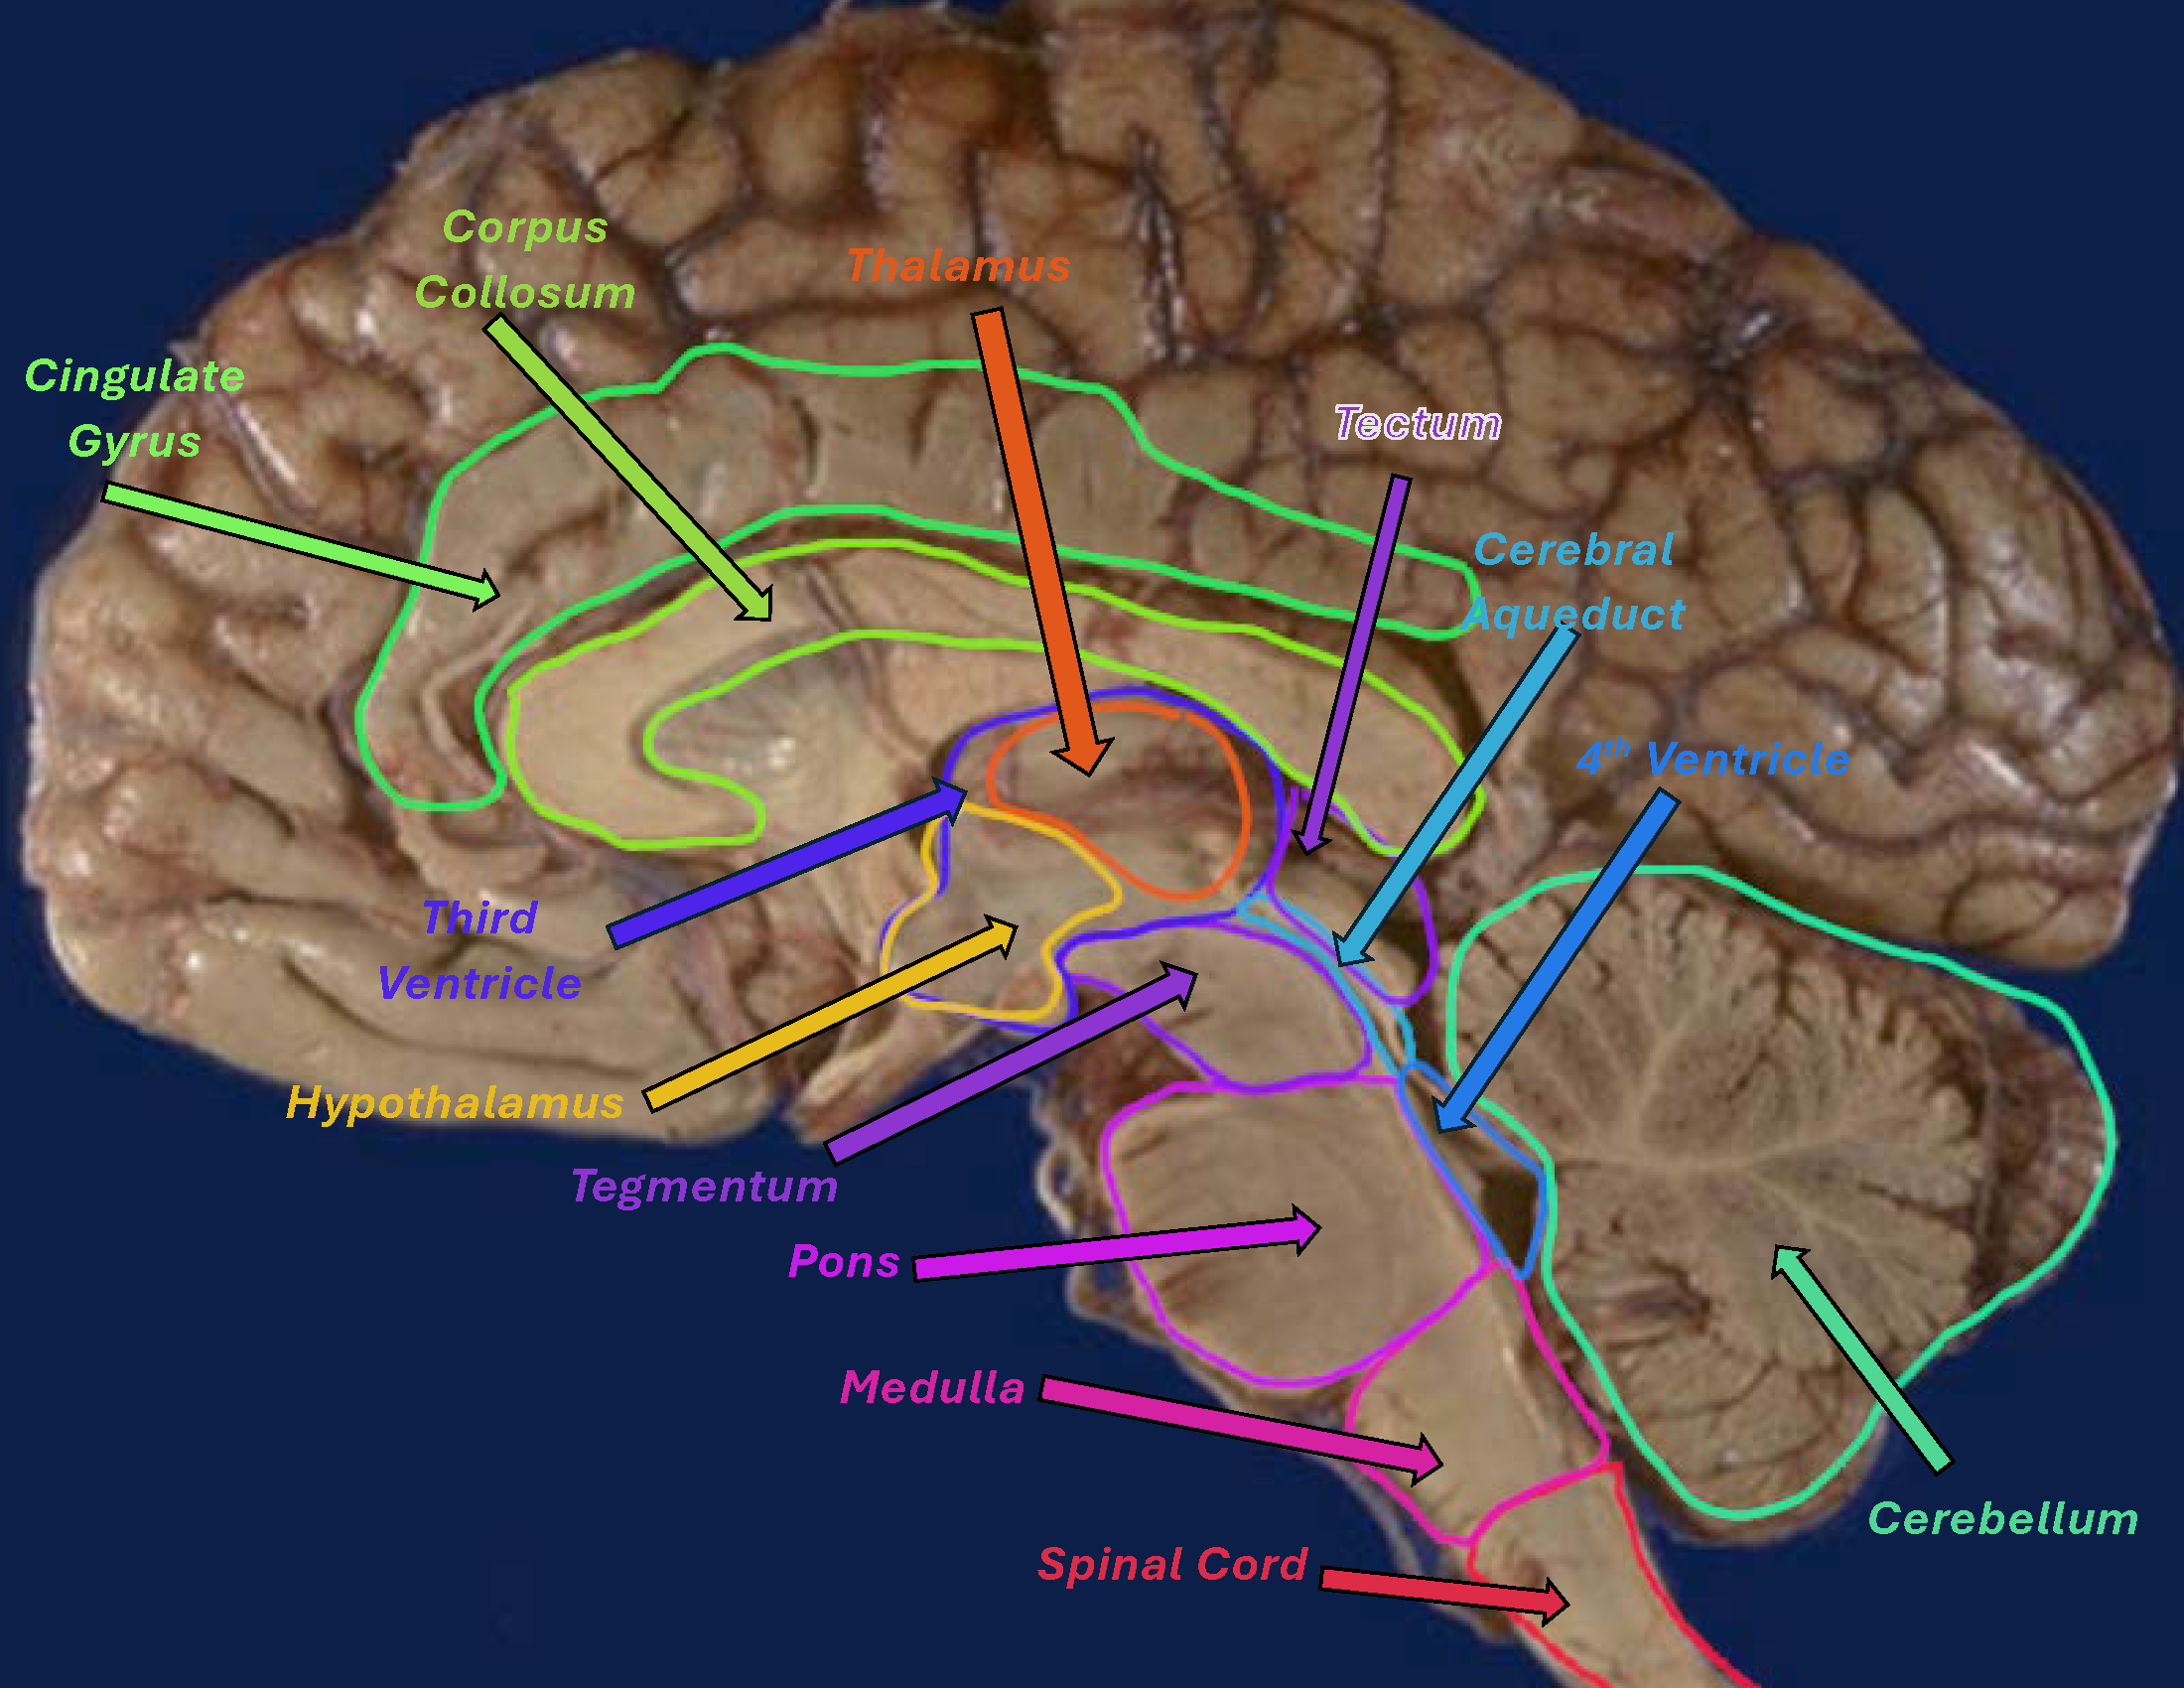
\includegraphics[width=.95\paperwidth,height=.95\paperheight,keepaspectratio]{images/midsagital_labeled.png}
%   \end{landscape}



% \chapter*{Exam 1b}
% \fancyhead[R]{Exam 1b}
% \addcontentsline{toc}{chapter}{Exam 1b}
% \vspace*{-0.25in}
% \section*{External Surface Structures}
\begin{itemize}
    \item \cyanit{Ansate Sulcus / Cruciate Fissure} - Located on the dorsal surface, separating frontal and parietal lobes.
    \item \cyanit{Medial Longitudinal Fissure} - Runs along the midline, separating the two cerebral hemispheres.
    \item \cyanit{Cerebellum} - Located at the posterior base of the brain.
    \item \cyanit{Coronal Sulcus / Superior Frontal Sulcus} - Found on the dorsal aspect, part of the frontal lobe.
    \item \cyanit{Transverse Fissure} - Separates the cerebellum from the cerebrum.
    \item \cyanit{Anterior / Rostral} - Toward the front of the brain.
    \item \cyanit{Posterior / Caudal} - Toward the back of the brain.
    \item \cyanit{Medial} - Toward the midline of the brain.
    \item \cyanit{Lateral} - Away from the midline.
\end{itemize}

\section*{Ventral Structures}
\begin{itemize}
    \item \cyanit{Olfactory Bulb} - Located at the most anterior portion of the ventral side.
    \item \cyanit{Cerebral Peduncle} - Found on the ventral midbrain, connects the cerebrum to the brainstem.
    \item \cyanit{Pons} - Bulging structure on the brainstem, anterior to the medulla.
    \item \cyanit{Pyramids on the Medulla} - Located on the ventral surface of the medulla oblongata.
    \item \cyanit{Spinal Cord} - Extends from the medulla caudally.
    \item \cyanit{Optic Chiasm} - X-shaped structure where optic nerves partially cross.
    \item \cyanit{Median Eminence / Tuber Cinereum} - Located at the base of the hypothalamus.
    \item \cyanit{Mammillary Body} - Small round structures part of the limbic system, posterior to the hypothalamus.
    \item \cyanit{Periamygdaloid Cortex / Uncus} - Located in the medial temporal lobe, part of the piriform cortex.
    \item \cyanit{Entorhinal Cortex} - Medial portion of the temporal lobe, key in memory processing.
    \item \cyanit{Lateral Olfactory Tract} - Extends from the olfactory bulb along the ventral surface.
    \item \cyanit{Rhinal Fissure} - Separates the neocortex from the piriform cortex.
    \item \cyanit{Insula / Island of Reil} - Located deep within the lateral sulcus.
    \item \cyanit{Sylvian Fissure} - Separates the temporal lobe from the frontal and parietal lobes.
\end{itemize}

\section*{Midbrain and Hindbrain Structures}
\begin{itemize}
    \item \cyanit{Superior Colliculus} - Dorsal midbrain, involved in visual processing.
    \item \cyanit{Inferior Colliculus} - Below the superior colliculus, involved in auditory processing.
    \item \cyanit{Pineal Body} - Small endocrine gland, located dorsally near the thalamus.
    \item \cyanit{Hypothalamus} - Located below the thalamus, controls endocrine functions.
    \item \cyanit{Corpus Callosum} - Large fiber bundle connecting the two cerebral hemispheres.
    \item \cyanit{Cingulate Gyrus} - Located superior to the corpus callosum, involved in emotion regulation.
    \item \cyanit{Cerebral Aqueduct} - Connects the third and fourth ventricles, running through the midbrain.
    \item \cyanit{Tegmentum} - Ventral part of the midbrain, involved in motor control.
    \item \cyanit{Massa Intermedia of the Thalamus} - Connects the two halves of the thalamus.
    \item \cyanit{Fornix} - White matter tract connecting the hippocampus to the hypothalamus.
\end{itemize}

\section*{Limbic System and Deep Brain Structures}
\begin{itemize}
    \item \cyanit{Hippocampus} - Located in the medial temporal lobe, essential for memory formation.
    \item \cyanit{Amygdala} - Anterior to the hippocampus, involved in emotion processing.
    \item \cyanit{Fimbria} - White matter tract leading from the hippocampus.
    \item \cyanit{Caudate Nucleus} - Part of the basal ganglia, involved in motor control.
    \item \cyanit{Lateral Ventricle} - Space within the corpus callosum, part of the ventricular system.
    \item \cyanit{Third Ventricle} - Space located between the two halves of the diencephalon.
\end{itemize}

% \begin{landscape}
%     \pagestyle{plain}
%     % \pagecolor{brainbackground}
%     \centering
%     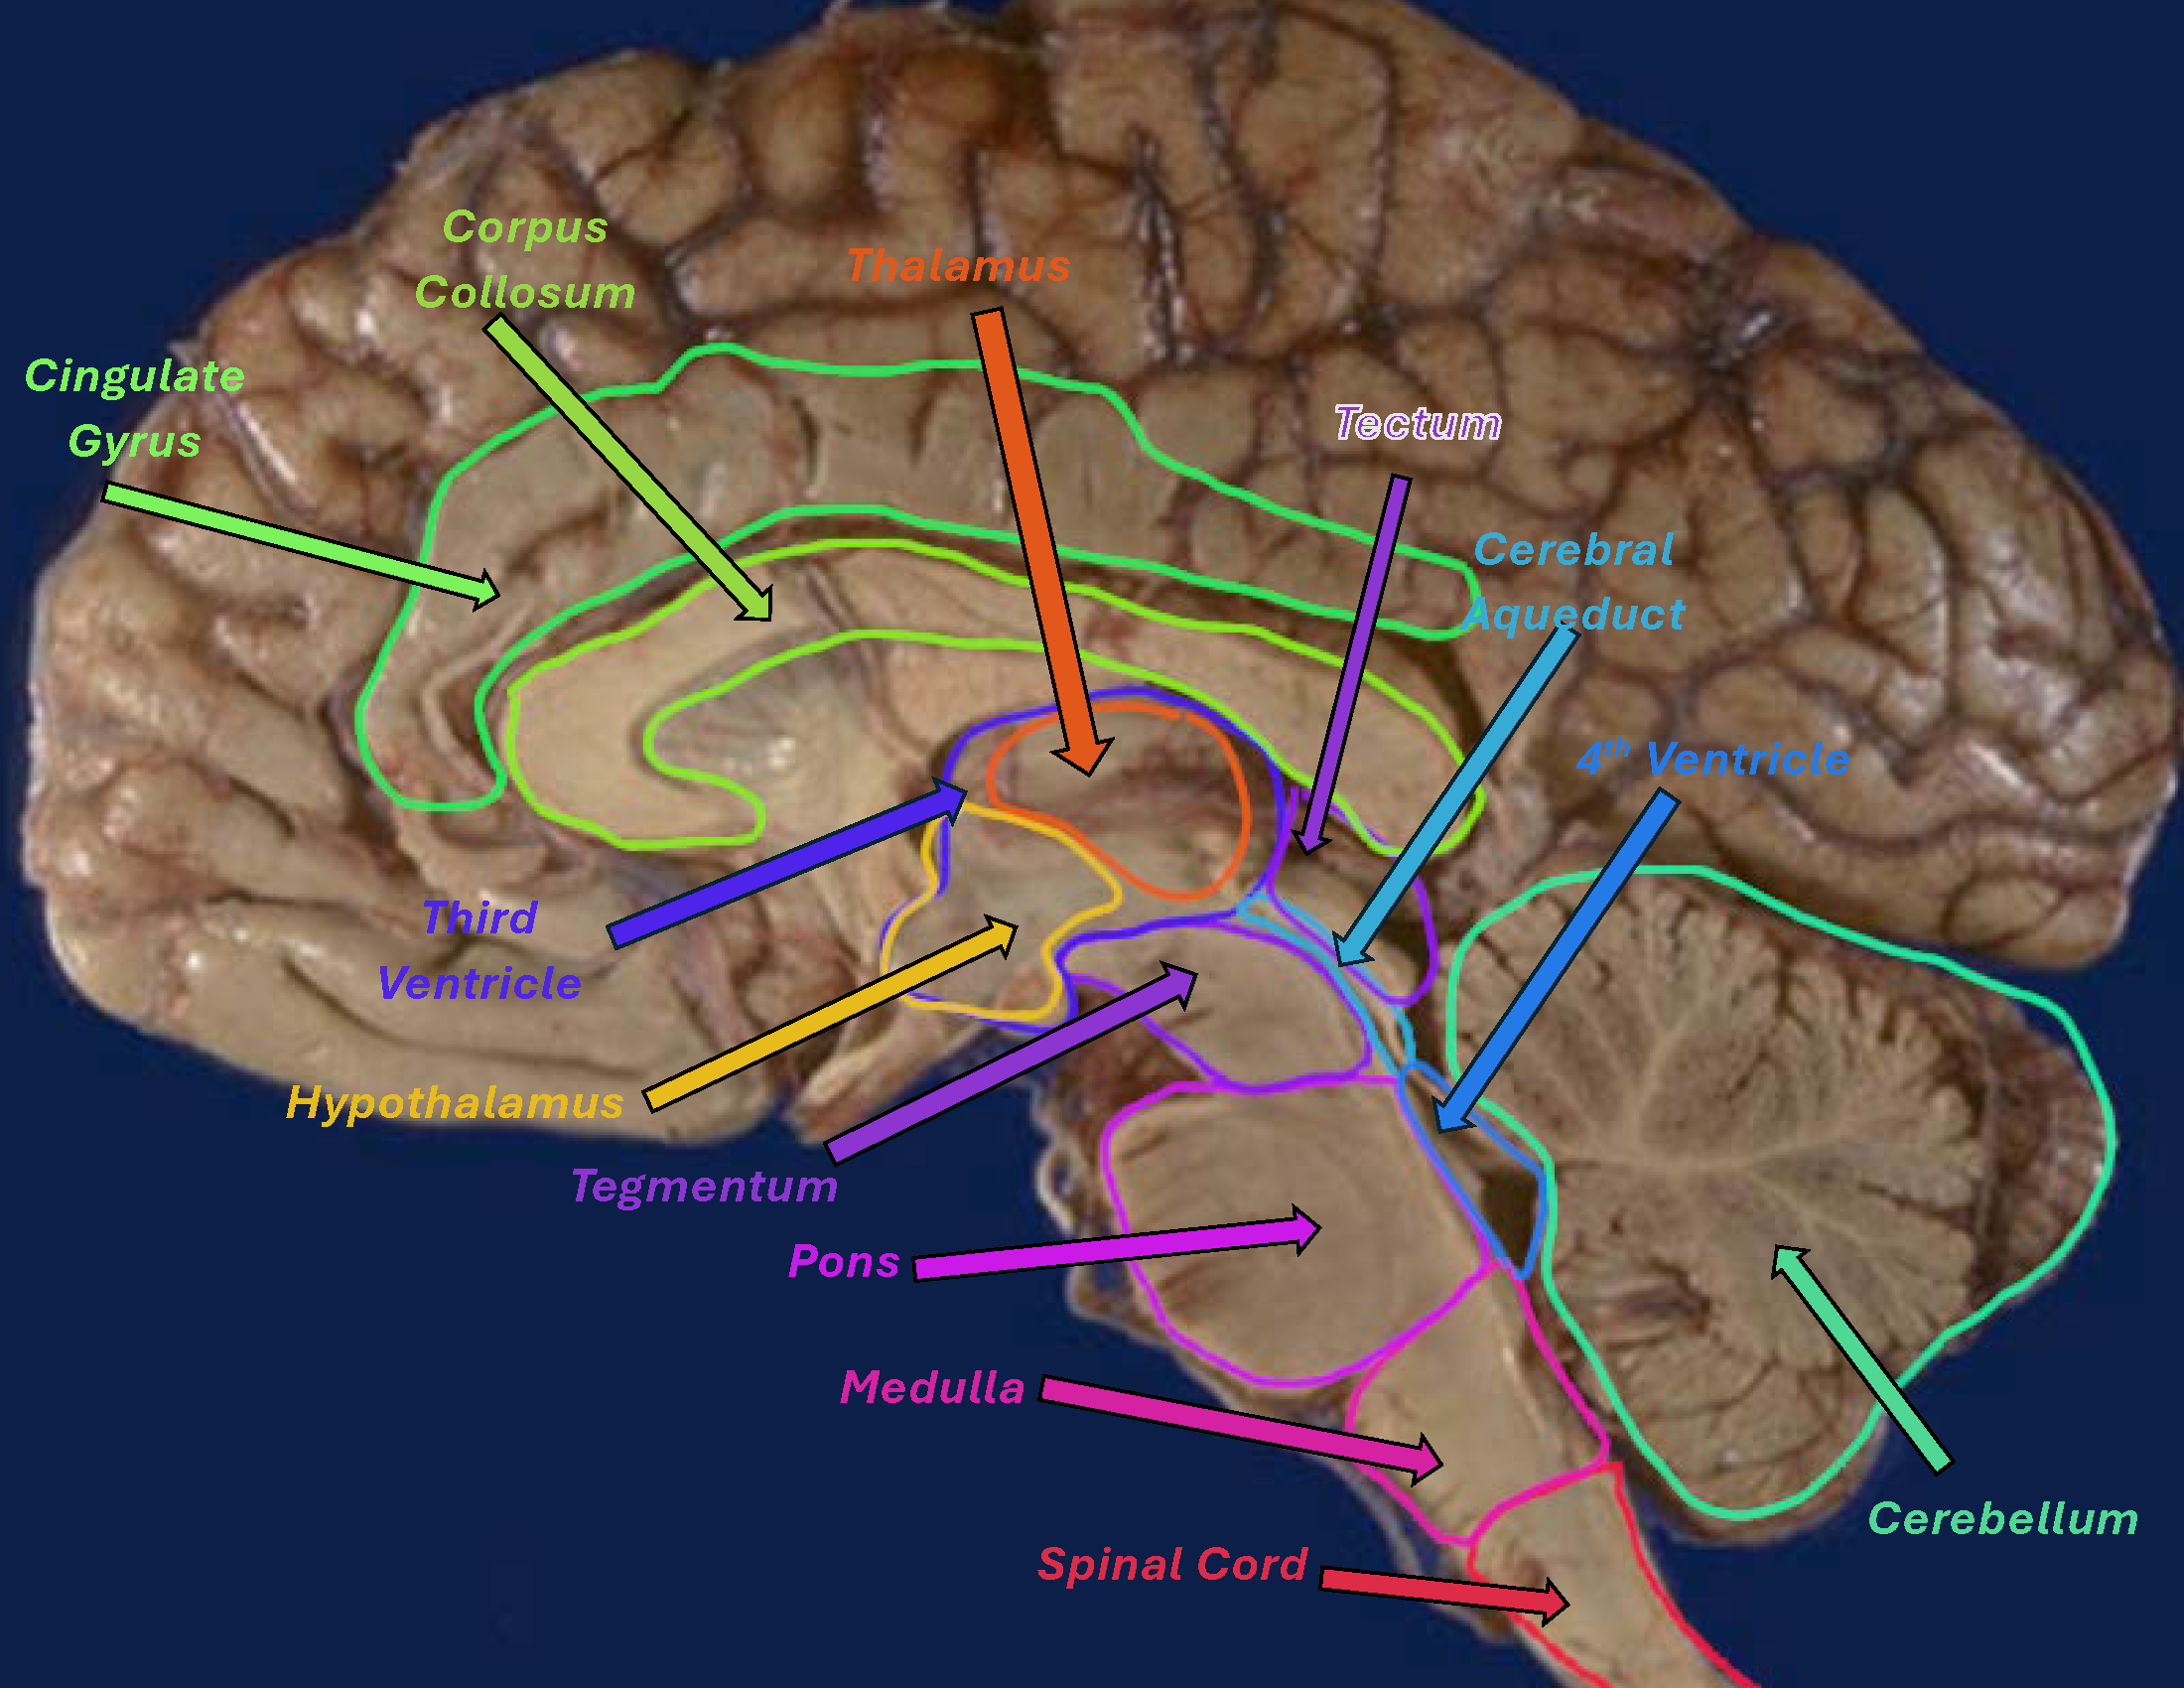
\includegraphics[width=.95\paperwidth,height=.95\paperheight,keepaspectratio]{images/midsagital_labeled.png}
%   \end{landscape}

\chapter*{Behavioral Lab}
\vspace*{-0.25in}
\begin{center}
    \textbf{We're starting with three studies:}
\end{center}

\begin{enumerate}
    \item \textbf{Study 1:} Blinking:
    \begin{coloredlist}
        \item Three levels of blinking:
        \begin{coloredlist}
            \item Reflexive blinking. Ex: When a puff of air is directed at the eye.
            \item Voluntary blinking. Ex: When you're asked to blink.
            \item Endogenous blinking. Meaning: ``originating from or due to internal causes.''
        \end{coloredlist}
        \item \cyanit{Endogenous blinking} is the focus of this study.
        \begin{coloredlist}
            \item Endogenous blinks occur during reading or speaking and reflect changes of attention and changes in thought processes. The more attention required by a visual task; the fewer endogenous blinks occur.
            \item More attention required is associated with fewer endogenous blinks. Especially for visual tasks.
            \item \textbf{The harder the tasks \(\rightarrow\) the fewer the blinks.}
            \item Even when a task is not visual, there is a decrease in endogenous blink rate (EBR) during a difficult task followed by flurry of blinks when task is over.
            \item \textbf{But wait!}
            \begin{coloredlist}
                \item EBR has been shown to increase when a cognitive secondary task is performed concurrently, and the cognitive task does not involve visual attention.
            \end{coloredlist}
            \item \textbf{WHY?}
            \begin{coloredlist}
                \item EB is a dopaminergic activity.
                \item Dopamine plays a big role in selective attention.
            \end{coloredlist}
        \end{coloredlist} 
        \item Through this study, we learned that endogenous blinking (DV) is affected by cognitive load (IV)
    \end{coloredlist}
    \item \textbf{Study 2:} Cartoon Judgement:
    \begin{coloredlist}
        \item Group 1 and 2 membership.
        \item Follow group instructions then rate the 3 cartoons that follow on scale from 1-10.
        \begin{coloredlist}
            \item 1 is NOT funny
            \item 10 is VERY funny
            \item Answers (Lips = Pen in lips; Teeth = Pen in teeth):

            \begin{tabular}[htbp]{ccccc}
                \toprule
                \textbf{Groups} & \textbf{Pics 1} & \textbf{Pics 2} & \textbf{Pics 3} & \textbf{Average} \\ \midrule
                \textbf{Lips} & 3 & 3 & 4 & \(3\frac{1}{3}\) \\ \midrule
                \textbf{Teeth} & 4 & 4 & 3 & \(3\frac{2}{3}\) \\ \midrule
                \textbf{Stretch} & 4 & 5 & 6 & 5 \\ \midrule
                \textbf{J. Jacks} & 4 & 2 & 3 & 3 \\ \bottomrule
            \end{tabular}

        \end{coloredlist}
        \item \textbf{Facial Feedback Hypothesis}
        \begin{coloredlist}
            \item Selective activation or inhibition of facial muscles has a strong impact on emotional responses to stimuli.
            \item Zygomatic major muscle.
            \begin{coloredlist}
                \item When we had the pen in our teeth, we were activating the zygomatic major muscle.
                \item This muscle is responsible for smiling.
            \end{coloredlist}
            \item Our data supported this hypothesis with a probability of \(p < 0.02\).
        \end{coloredlist}
        \item \textbf{Arousal}
        \begin{coloredlist}
            \item Increased heart rate in many emotions.
            \item Heart rate and attraction
            \begin{coloredlist}
                \item 1973 Dutton and Aron
                \begin{coloredlist}
                    \item Shaky high bridge vs. low stable bridge.
                    \item Woman on the other side who is asking questionnaire questions (faux DV).
                    \item She gave her phone number to the guys once they got done answering the questions.
                    \item The actual DV was the amount of phone calls she received and the sexual content in questionnaire answers.
                    \item The high bridge group had more sexual content in their messages.
                \end{coloredlist}
                \item 15 minutes of physical activity, then rate attractiveness of potential mates.
            \end{coloredlist}
        \end{coloredlist}
    \end{coloredlist}
\end{enumerate}

\cyanit{Psychophysiology:} Behavioral, cognitive, emotional, and social events are all mirrored in physiological processes. \\

The idea is that we can get a peep into your psychology by looking at what your biology is doing. \\

\textbf{Sleep:} EEG (Electroencephalogram; measuring brain activity), EOG (Electrooculogram; measuring eye movement), EMG (Electromyography; measuring muscle movement), ERP (Event-Related Potential; measuring event-related potential). \\ 

When your brain is hooked up to the ERP and you are asked either task relevant-stimulus, important stimulus, or surprising stimulus, it will produce a higher \(p\)\textemdash300 amplitude compared to otherwise. Think about how this would be used for interrogating a suspect, for example. \\ 

Then, there are \(n\)\textemdash350 amplitudes which are activated when we are asleep, and we hear our name, for example. \\

Notice the implications of this with sleeping: the more tired you are (or closer to falling asleep), the harder it will be to find the \(p\)\textemdash300 amplitude. \\

\cyanit{Omitted Stimulus Paradigm} -- Given a constant stimulus, this is the phenomena wherein there is a gap in the pattern. This will result in a higher \(p\)\textemdash300 amplitude. \\

\textbf{Polygraph:} Respiration, GSR (EDA), Blood flow, Blood pressure, and heart rate. \\

With a polygraph, we're looking at all the components of the peripheral nervous system. That is, when we're ``looking at  '' a polygraph, we're not measuring lying, but all the physiological responses that are associated with lying. \\



\section{EDA}

\begin{coloredlist}
    \item \cyanit{Electrodermal Activity}
    \begin{coloredlist}
        \item Old name: Galvanic Skin Response
        \item Measuring sympathetic nervous system activity by detecting sweat gland activity by measuring the conductance of an electrical signal from one electrode to another.
        \item More rapid conductance with more activity.
        \item Particularly good for emotion.
        \item Maybe attention.
        \item This also is a good measure for the sympathetic nervous system because it is the only one that can enervate the sweat glands.
    \end{coloredlist}
\end{coloredlist}

\subsection{What if I Want to Know}

\begin{coloredlist}
    \item If you're lying
    \item Cognitive or emotional states when you're sleeping
    \item If you're attending to stimuli I'm presenting
\end{coloredlist}

\textbf{Psychophysiology is different from Physiological Psychology}. Note that Psychophysiology is where mind/behavior is the IV, and physiology is the DV. Similarly, Physiological Psychology uses the same IVs and DVs, but notice that we are manipulating the physiological psychology to measure psychology. Remember the independent variable is first (mnemonic). \\

\subsubsection{Examples}

\begin{coloredlist}
    \item Present snake photo or not. Then measure effects on physiology that evidence fear.
    \item Presenting in-group and out-group photographs. Then measure effects on physiology that evidence prejudicial cognition.
    \item Drugs: Measure effects on psychology (behavior/aggression)
    \item Lesion: Measure effects on psychology (cognition/memory)
    \item Manipulate heart rate: (behavior/attractiveness ratings)
    \item Electrical Stim of Brain [tDCS (transcranial direct current stimulation)]: Measure effects on psychology (mood/emotion/depression)
\end{coloredlist}

\section{EEG}

\begin{coloredlist}
    \item Activity in large groups of neurons.
    \item Difference in electrical activity at a reference point and site of interest.
    \item You get: Wavelike patterns.
    \item \cyanit{International 10-20 system}.
    \begin{coloredlist}
        \item Fz, Fp1, Fp2, F7, F8, F3, F4, T3, T4, Cz, C3, C4, T5, T6, Pz, P3, P4, O1, O2.
        \begin{multicols}{2}
            \begin{coloredlist}
                \item F = Frontal
                \item T = Temporal
                \item C = Central
                \item P = Parietal
                \item O = Occipital
                \item Odd numbers = left hemisphere.
                \item Even numbers = right hemisphere.
                \item Z = Midline
            \end{coloredlist}
        \end{multicols}
    \end{coloredlist}
    \item Researchers use \cyanit{visual inspection} to look at the EEG data.
    \item Measurements
    \begin{coloredlist}
        \item \cyanit{Frequency} -- \(\frac{1}{\text{time}}\) (in Hz)
        \item \cyanit{Amplitude} -- Height of wave (in \(\mu \text{V}\))
    \end{coloredlist}
\end{coloredlist}

\section{Neurofeedback}

\begin{coloredlist}
    \item Learn to control your brain activity.
    \begin{coloredlist}
        \item See the activity
        \item Get reinforcement or punishment
        \item Make changes
        \item Even if you don't ``know'' what you're doing, you can still learn to control your brain activity.
    \end{coloredlist}
\end{coloredlist}









%-%-%-%-%-%-%-%-%-%-%-%-%-%-%-%-%-%-%-%-%-%-%-%-%-%-%-%-%-%-%-%-%-%-%-%-%-%-%
\end{document}
%-%-%-%-%-%-%-%-%-%-%-%-%-%-%-%-%-%-%-%-%-%-%-%-%-%-%-%-%-%-%-%-%-%-%-%-%-%-%

%-%-%-%-%-%-%-%-%-%-%-%-%-%-%-%-%-%-%-%-%-%-%-%-%-%-%-%-%-%-%-%-%-%-%-%-%-%-%